\documentclass[11pt]{article}
\usepackage[utf8]{inputenc}
\usepackage[T1]{fontenc}
\usepackage{lmodern}
\usepackage[margin=1in]{geometry}
\usepackage{amsmath,amssymb,amsthm,mathtools}
\usepackage{graphicx}
\usepackage{booktabs}
\usepackage{multirow}
\usepackage{xcolor}
\usepackage{colortbl}
\usepackage{caption}
\usepackage{subcaption}
\usepackage{enumitem}
\usepackage{microtype}
\usepackage{tcolorbox}
\usepackage[hidelinks]{hyperref}

\definecolor{good}{HTML}{E8F0EA}
\definecolor{bad}{HTML}{F8D7DA}
\definecolor{warn}{HTML}{FFF2CC}
\newcommand{\code}[1]{\texttt{\small #1}}
\newtheorem{definition}{Definition}
\newtheorem{property}{Property}
\newtcolorbox{algbox}[1]{colback=gray!4,colframe=gray!55,title={#1},
  fonttitle=\bfseries\small,boxrule=0.4pt,left=4pt,right=4pt,top=3pt,bottom=3pt}
\captionsetup{font=small}

\title{\textbf{A Shared Intelligence Network for Employment-Experience Fraud:\\
Privacy-Preserving Signal Sharing and Incentive Design}}
\author{Vijay Javvadi\\
\small Independent Researcher\\
\small \texttt{jvijayprasad@gmail.com}}
\date{Preprint, June 2026}

\begin{document}
\maketitle

\begin{abstract}
\noindent Misrepresentation of professional experience---fabricated seniority,
invented employment timelines, and false credentials---is one of the most common
and least-policed forms of hiring fraud, and generative models that mass-produce
convincing synthetic candidates are lowering its cost to near zero. Two mature
bodies of work bear on the problem but have never been combined for hiring:
machine-learning detection of inconsistent r\'esum\'es, and the
privacy-preserving fraud \emph{consortia} that banking and cybersecurity use to
pool bad-actor signals across institutions. Today every employer screens in
isolation, so a fraudster rejected by one organization simply re-applies to the
next under a new identity, with no shared memory. We present a framework for an
\emph{employment-fraud intelligence network} that integrates three threads the
literature has studied separately: (i) layered detection that pairs a
deterministic, explainable timeline-impossibility engine with inferential
signals; (ii) privacy-preserving cross-organization sharing, for which we give a
threat model and show---analytically and in simulation---that the naive
``publish a hash of the email and phone'' construction common in industry offers
\emph{no} anonymity, recovering 100\% of any candidate an adversary can
enumerate; and (iii) an incentive mechanism for voluntary contribution, for which
we identify and simulate an adverse-selection failure---paying more for
confirmed-fraud reports than for verified-legitimate ones corrupts the shared
data, driving the network false-positive rate from 0\% to 19\% as strategic
participation grows---and propose an outcome-symmetric, evidence-gated,
reputation-weighted correction that holds precision at 1.00. We treat regulatory
compatibility (FCRA, GDPR) as a first-class design constraint, quantify the
contributory-network flywheel and fraud-ring detection, and release a seeded,
reproducible implementation and evaluation harness as open source. All claims are
demonstrated on reproducible simulations and a public career-trajectory corpus;
commercial operation, which triggers the heaviest regulatory duties, is
deliberately deferred.
\end{abstract}

\noindent\textbf{Keywords:} employment fraud, r\'esum\'e fraud,
privacy-preserving data sharing, private set intersection, fraud consortia,
incentive mechanisms, mechanism design, hiring, FCRA, GDPR, responsible AI.

\tableofcontents
\newpage

\section{Introduction}\label{sec:intro}
Hiring decisions rest on a candidate's self-reported history, and that history is
increasingly fabricated. Industry surveys place the annual cost of r\'esum\'e
fraud in the hundreds of billions of dollars, report that a majority of
candidates embellish their experience, and find that only a minority of hiring
managers are confident they can detect it~\cite{resumefraud2025}. The most
damaging variant is not a polished bullet point but a fabricated \emph{timeline}:
a junior professional claiming a decade of seniority, an employment span that
pre-dates graduation, or a wholly synthetic identity assembled to pass automated
screening.

Two forces are widening the gap between fraud and defense. First, generative
models have collapsed the cost of fabrication: anyone can prompt a large language
model for a coherent r\'esum\'e, a matching cover letter, and interview-ready
answers, and adversarial agent frameworks can now synthesize entire, internally
consistent career trajectories~\cite{fakecareers2025,agentgen2025}. Second, and
more fundamentally, defenses \emph{do not share}. Background-screening vendors
verify identity, criminal history, and payroll records, and a growing literature
applies natural-language processing and anomaly detection to score r\'esum\'es
for inconsistency~\cite{resumefraud2025,resumeml}. But each employer operates
alone. A candidate flagged as fraudulent by one organization carries no warning
to the next; the fraudster re-applies elsewhere, often under a slightly altered
identity, and the second organization repeats the first's work and its mistakes.

Other risk-bearing industries solved exactly this coordination problem with
\emph{contributory networks}. Insurers pool claims data; banks and cybersecurity
teams share fraud and threat indicators across institutions; national schemes
such as the UK's Cifas National Fraud Database aggregate member-reported cases at
scale~\cite{cifas}. Crucially, the privacy-preserving variants of these networks
exchange signals without any raw personal data leaving a participant, using
federated learning or private set intersection
(PSI)~\cite{starlit2024,otpsi2026}. No equivalent shared layer exists for
employment fraud. This paper asks what one should look like.

\paragraph{Why this is hard, and why prior pieces do not suffice.}
A naive engineer might assume the recipe is obvious: detect fraud with a
classifier, share flags as hashes, and pay members to contribute. Each step
contains a trap that the separate literatures do not address \emph{in this
setting}. Detection that relies on inferential signals (digital footprint,
account age) has a high false-positive rate on atypical-but-genuine
candidates---privacy-conscious senior professionals, career changers, non-Western
career paths---and a false accusation in a \emph{shared} network is repeated and
amplified across employers. Sharing identifiers as hashes provides no privacy:
emails and phone numbers are low-entropy, so an adversary can enumerate and
match~\cite{cook2019,skyflow}. And paying more for ``confirmed fraud'' than for
``verified legitimate'' reports---the intuitive design, since fraud feels more
valuable---creates an adverse-selection loop that fills the network with weak
accusations. These failure modes interact: the incentive flaw manufactures the
inaccurate shared assessments that the privacy and legal constraints most
penalize.

\paragraph{Contributions.}
We make the following contributions, each developed as a design and validated on
reproducible experiments (Section~\ref{sec:results}):
\begin{enumerate}[leftmargin=1.5em,itemsep=2pt]
  \item \textbf{An integrated framework} (Sections~\ref{sec:arch}--\ref{sec:incentive})
  for an employment-fraud intelligence network that unifies layered detection,
  privacy-preserving sharing, and incentive-aligned contribution under explicit
  regulatory constraints.
  \item \textbf{A deterministic timeline engine} (Section~\ref{sec:detect}) that
  catches internally inconsistent claims with an explainable, near-zero
  false-positive rule set, and an empirical demonstration that it---alone---cannot
  catch internally consistent AI fabrications, motivating the other layers.
  \item \textbf{A privacy threat model and demonstration}
  (Sections~\ref{sec:privacy},~\ref{sec:reid}) proving that the industry-default
  hash construction recovers 100\% of enumerable candidates, with a re-id curve
  that scales linearly with adversary coverage, and a PSI-with-threshold
  alternative that bounds insider leakage.
  \item \textbf{An incentive analysis and mechanism}
  (Sections~\ref{sec:incentive},~\ref{sec:res:incentive}) that identifies,
  simulates, and corrects an adverse-selection failure specific to fraud
  consortia, with $95\%$ confidence intervals over $30$ seeds.
  \item \textbf{Two network-level results}
  (Sections~\ref{sec:res:flywheel},~\ref{sec:res:ring}): a quantified
  contributory-network flywheel (repeat-fraud catch rate rising with
  participation) and fraud-ring detection via shared-identifier linkage.
  \item \textbf{A regulation-as-architecture analysis} (Section~\ref{sec:legal})
  mapping FCRA and GDPR obligations onto concrete design decisions, and an
  open-source, seeded, reproducible release~\cite{truthhirecode}.
\end{enumerate}

\paragraph{Scope and honesty.} This is a framework paper. We formalize the
problem, analyze the design space, and demonstrate the detection, privacy,
incentive, and network properties on seeded simulations and a public
career-trajectory corpus. We do \emph{not} claim a deployed multi-organization
study; that, and the measurement of false-positive rates on real, atypical
candidates at population scale, is the central item of future work
(Section~\ref{sec:agenda}). We are explicit throughout about which results are
analytic, which are simulated, and which depend on data we generate versus data
we obtain.

\section{Background and Related Work}\label{sec:related}

\subsection{Detecting fabricated experience}
Automated r\'esum\'e-fraud detection extracts structured entities (degrees,
institutions, dates, employers, titles) and scores them for internal
inconsistency and against external sources using supervised or anomaly-detection
models~\cite{resumefraud2025,resumeml}. A recent thread targets machine-generated
candidates specifically: heterogeneous-graph models detect synthetic career
trajectories~\cite{fakecareers2025}, while agent-based generators demonstrate how
realistic such trajectories have become~\cite{agentgen2025}. These methods are
valuable but share two properties relevant here. They operate \emph{within a
single organization's data}, so they cannot exploit cross-employer recurrence;
and they lean on inferential, probabilistic features that, as we show
(Section~\ref{sec:res:agent}), are brittle against an adaptive adversary and
carry false-positive risk for atypical genuine candidates.

\subsection{Cross-organization fraud consortia}
Pooling fraud signals across institutions is well established in finance and
security. Cifas aggregates member-reported fraud at national
scale~\cite{cifas}. Privacy-preserving variants avoid sharing raw data: federated
learning trains shared fraud models without centralizing
records~\cite{starlit2024}. The employment domain has no comparable
infrastructure, and---as Section~\ref{sec:incentive} argues---naively importing
the financial-consortium playbook would import an incentive structure that is
actively harmful when the shared signal is a derogatory accusation about an
individual job-seeker.

\subsection{Private set intersection and the limits of hashing}
Private set intersection lets parties compute the intersection of their sets
without revealing the non-intersecting elements; over-threshold and multi-party
variants reveal only elements shared by at least $t$ participants~\cite{otpsi2026}.
These are the right primitive for a sharing layer. The wrong primitive---and the
industry default---is to publish a hash of an identifier. Hashing fails to
anonymize when the input space is enumerable: emails, phone numbers, and names
are low-entropy, so an adversary can hash every candidate value and
match~\cite{cook2019,skyflow}. Salting helps only if the salt is secret and
unshared, which defeats cross-party matching; Bloom filters~\cite{bloom1970}
reduce storage but are themselves brute-forceable at small budgets. We make this
concrete in Section~\ref{sec:reid}.

\subsection{Incentivizing data contribution}
Consortia function only if members contribute, and the data-sharing-market
literature formalizes how to elicit data value and compensate contribution so
that sustainable consortia form~\cite{datasharing2023}; surveys catalog monetary,
reputational, and access-based incentives. Fraud networks add a domain-specific
hazard we make precise in Section~\ref{sec:incentive}: because the reward is
attached to a \emph{verdict} the contributor itself supplies, the mechanism can
be gamed by the very reports it solicits.

\subsection{Gap}
Detection, private sharing, and incentive design have each been studied in
isolation, and largely outside hiring. No prior work integrates them into a
regulation-aware employment-fraud network, nor analyzes the privacy and incentive
failure modes specific to that setting. That integration, and the demonstration
of those failure modes and their corrections, is our contribution.

\subsection{Identity verification and algorithmic hiring}
Two adjacent literatures bound the problem. Identity-proofing and
document-verification systems establish \emph{who} a candidate is but not whether
their claimed \emph{history} is real; they are complementary to, not substitutes
for, timeline analysis. Separately, a growing body of work on algorithmic hiring
fairness documents how automated screening can encode and amplify bias against
protected and non-standard groups. That literature is the reason our inferential
and network layers are advisory rather than dispositive: a probabilistic signal
that correlates with a non-standard career path must never, by itself, end a
candidacy. We treat fairness not as a post-hoc audit but as a constraint that
shapes where automation is permitted to act.

\section{Problem Definition and Threat Model}\label{sec:threat}
We formalize the setting before describing the system.

\begin{definition}[Candidate record]
A candidate record is a tuple $r=(\mathrm{id}, a, g, J, y)$ where $\mathrm{id}$ is
a set of identifiers (name, email, phone), $a$ is age, $g$ is graduation year,
$J=\{(s_i,e_i,\tau_i)\}$ is a set of job intervals with start $s_i$, end $e_i$,
and employment type $\tau_i$, and $y$ is total claimed years of experience.
\end{definition}

\begin{definition}[Experience-fabrication fraud]
A record exhibits experience-fabrication fraud if its timeline could not have been
truthfully accrued: $y > a-18$ (impossible seniority); $\min_i s_i < g$
(pre-graduation employment); overlapping full-time intervals; $y$ exceeding
$\sum_i (e_i-s_i)$ beyond tolerance (inflation); a non-existent employer; or a
wholly synthetic identity.
\end{definition}

\begin{definition}[Participating organization]
A participating organization screens candidates and may contribute and query
\emph{signal records} to a shared network. A signal record references a candidate
by privacy-protected identifiers and carries an outcome label and the flag codes
that fired---never raw personal data, documents, or employer-specific detail.
\end{definition}

We assume three adversaries.

\noindent\textbf{Candidate adversary $\mathcal{A}_C$.} Seeks a low risk score and
progression to interview. May generate documents and a digital footprint with AI,
re-apply across organizations, and vary identifiers across applications (a
\emph{fraud ring} when one actor uses many identities).

\noindent\textbf{Privacy adversary $\mathcal{A}_P$.} An honest-but-curious
participant (or a breach of one) that follows the protocol but tries to
re-identify candidates in shared data or learn another organization's applicants.
The security goal is that a signal record must not let $\mathcal{A}_P$ recover the
identity or hiring history of a candidate it has not itself seen.

\noindent\textbf{Incentive adversary $\mathcal{A}_I$.} A self-interested
participant that maximizes its own benefit (cheaper or better screening) and may
submit low-quality, duplicate, or strategically biased reports if rewarded. The
mechanism-design goal is that the network's outputs remain accurate under a
bounded fraction of such participants.

\begin{property}[Design goals]\label{prop:goals}
The system should (G1) catch internally inconsistent fraud deterministically and
explainably; (G2) leak no more than membership, and only above a corroboration
threshold, to $\mathcal{A}_P$; (G3) keep network precision high under
$\mathcal{A}_I$; and (G4) make only advisory, disputable, human-reviewable
recommendations, never automated adverse decisions, in deference to FCRA/GDPR.
\end{property}

\section{System Architecture}\label{sec:arch}
The system is a four-layer pipeline producing, for each candidate, an explainable
set of flags and an advisory risk indication, plus an optional contribution to
the shared network. Figure~\ref{fig:layers} previews how detection responsibility
divides across layers: the deterministic layer fully covers internally
inconsistent claims, while internally consistent AI fabrications fall to the
inferential layer.

\begin{figure}[t]\centering
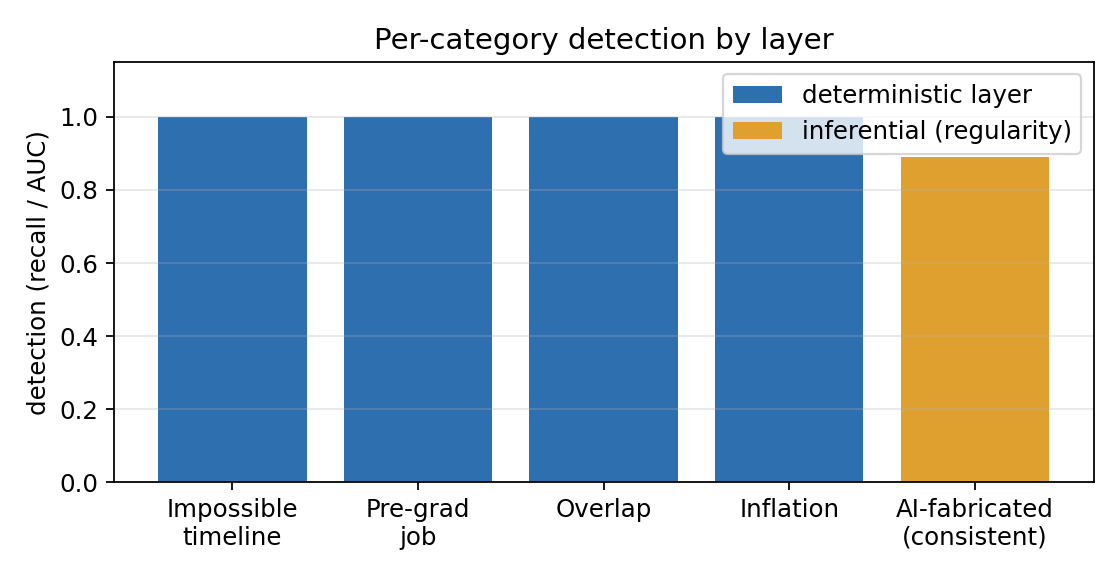
\includegraphics[width=0.74\linewidth]{figures/fig_layers.png}
\caption{Per-category detection by layer. The deterministic layer covers the four
impossibility classes; internally consistent AI-fabricated identities require the
inferential layer (Section~\ref{sec:res:agent}).}\label{fig:layers}
\end{figure}

Layer~1 (deterministic) tests internal logical consistency and needs no external
data. Layer~2 (inferential) draws on digital footprint, account age, web
presence, and employer-registry existence---advisory, probabilistic signals.
Layer~3 (network) contributes and queries the shared intelligence layer. Layer~4
(governance), threaded through the others, enforces the advisory, disputable,
audited posture required by Property~\ref{prop:goals}(G4). Sections~\ref{sec:detect}
through~\ref{sec:incentive} describe the layers that carry novel content.

\section{Detection Layers}\label{sec:detect}

\subsection{The deterministic timeline engine}\label{sec:det}
The first layer is deliberately not machine learning. It applies a small set of
logical-consistency rules to the candidate's \emph{own} claims, so it is
explainable, parameter-light, and has a near-zero false-positive rate: it fires
only on self-contradiction, independent of lifestyle, geography, or digital
footprint. Algorithm~1 states the core.

\begin{algbox}{Algorithm 1: \textsc{TimelineScore}$(r)$}
\ttfamily\small
\textbf{input} record $r=(\mathrm{id},a,g,J,y)$;\ \textbf{output} score, flags\\[2pt]
score $\leftarrow 0$;\ flags $\leftarrow \emptyset$\\
\textbf{if} $a$ defined and $y > a-18$:\ \ score $\mathrel{+}= 50$;\ add \code{TIMELINE\_IMPOSSIBLE}\\
\textbf{if} $g$ defined and $\min_i s_i < g$:\ \ score $\mathrel{+}= 40$;\ add \code{JOB\_BEFORE\_GRADUATION}\\
$O \leftarrow$ \#\,pairs of full-time intervals overlapping $> \theta_o$ months\\
\textbf{if} $O>0$:\ \ score $\mathrel{+}= 25\,O$;\ add \code{EMPLOYMENT\_OVERLAP}\\
\textbf{if} $y > \sum_i(e_i-s_i)+\theta_y$:\ \ score $\mathrel{+}= 25$;\ add \code{EXPERIENCE\_INFLATION}\\
\textbf{return} $\min(\text{score},100)$, flags
\end{algbox}

Here $\theta_o$ (overlap tolerance, months) and $\theta_y$ (inflation tolerance,
years) absorb benign transitions and rounding. Missing fields cause the
corresponding rule to abstain rather than fire, so the engine degrades gracefully
on partial r\'esum\'es. The weights derive from severity, not from training, and
the final score is capped at 100.

\subsection{Inferential signals}\label{sec:infer}
The second layer adds coverage the first cannot: it scores digital footprint,
account age, corroborating web presence, and employer-registry existence. These
signals are probabilistic and, as Section~\ref{sec:res:agent} shows, both brittle
against adaptive adversaries and false-positive-prone for privacy-conscious
genuine candidates. We therefore treat them strictly as \emph{advisory} inputs to
human review (Property~\ref{prop:goals}(G4)), never as automated-rejection
triggers.

\subsection{The network signal}\label{sec:netsig}
The third layer queries the shared network: has this candidate been reported by
other organizations, and by how many? Its value is the cross-employer memory
absent today. Its difficulty is that the query and the contribution must preserve
privacy (Section~\ref{sec:privacy}) and resist gaming (Section~\ref{sec:incentive}).

\section{Privacy-Preserving Sharing}\label{sec:privacy}

\subsection{Why the industry default fails}
A natural design publishes $H(\text{email}\,\|\,\text{phone})$ for a fixed hash
$H$. Because email and phone are low-entropy, $\mathcal{A}_P$ holding a candidate
list (e.g., its own applicant pool) computes the same hashes and re-identifies
everyone in the shared set. The hash is obfuscation, not anonymity; ``we only
store hashes'' is not a sound privacy claim. Section~\ref{sec:reid} quantifies
this: re-identification equals adversary coverage and reaches 100\% at full
enumeration.

\subsection{A membership protocol with a disclosure threshold}
We frame sharing as private set membership rather than publication. Candidate
references are compared through a PSI protocol that reveals only whether a match
exists, gated on a corroboration threshold $t$: a network concern is disclosed
only when at least $t$ independent organizations have reported the same candidate
(Algorithm~2). Thresholding serves two ends at once---it raises the
evidentiary bar before any derogatory signal is surfaced, and it bounds what any
single participant can learn.

\begin{algbox}{Algorithm 2: \textsc{ThresholdQuery}$(\mathrm{id}, t)$}
\ttfamily\small
\textbf{each org} encodes its reported candidates under a PSI protocol $\Pi$\\
$c \leftarrow \Pi.\textsc{CountMatches}(\mathrm{id})$\ \ (\#orgs reporting id; no identities revealed)\\
\textbf{if} $c \ge t$:\ \textbf{return} \code{NETWORK\_FLAG}$(c)$\ \ \textbf{else} \textbf{return} \code{none}
\end{algbox}

Where a lighter-weight deployment is required, a keyed construction (an HMAC under
a network-secret pepper) with rate-limited, audited lookups raises the attacker's
cost. As Section~\ref{sec:reid} shows, however, keying defeats only an
\emph{outside} adversary: a consortium insider holding the key recovers
everything, so keying is a breach mitigation, not a privacy guarantee. The
operative design principle is therefore invariant to the chosen primitive:
\emph{treat every shared reference as re-identifiable personal data, and minimize
what a match discloses.}

\section{Incentive Mechanism}\label{sec:incentive}

\subsection{Credits and the adverse-selection trap}
To bootstrap contribution, a consortium can grant \emph{credits} that offset a
member's screening costs---a concrete instance of compensating contribution to
sustain a data-sharing consortium~\cite{datasharing2023}. The hazard is the
reward schedule. A schedule that pays \emph{more} for a ``confirmed fraud'' report
than for a ``verified legitimate'' one creates an adverse-selection loop:
participants are incentivized to label borderline candidates as fraud, the shared
set fills with weakly substantiated accusations, the network false-positive rate
rises, and the outputs become both less accurate and more legally hazardous
(Section~\ref{sec:legal}). Section~\ref{sec:res:incentive} demonstrates this:
under the naive schedule, the network false-positive rate climbs from $0\%$ to
$19\%$ as strategic participation grows to $50\%$.

\subsection{Three corrections}
We propose three corrections that move the mechanism from rewarding
\emph{verdicts} to rewarding \emph{verified information}:
\begin{description}[leftmargin=1.2em,itemsep=2pt]
  \item[(i) Outcome symmetry.] Reward any verified, audited outcome equally, so
  confirming innocence is as valuable as confirming fraud, removing the farming
  incentive.
  \item[(ii) Evidence gating.] A report contributes to a network-visible concern
  only with qualifying evidence and corroboration to threshold $t$.
  \item[(iii) Reputation weighting.] Weight a participant's contributions by the
  historical accuracy of its reports (Algorithm~3), so that
  strategically noisy reporting decays in influence.
\end{description}

\begin{algbox}{Algorithm 3: reputation update}
\ttfamily\small
\textbf{init} $\mathrm{rep}[p] \leftarrow 1$ for each participant $p$\\
\textbf{on} adjudicated outcome $o$ for a report $(p,\ell)$:\\
\hspace*{1.2em}$\mathrm{agree}[p] \mathrel{+}= [\ell = o]$;\ \ $\mathrm{total}[p] \mathrel{+}= 1$\\
\hspace*{1.2em}$\mathrm{rep}[p] \leftarrow \mathrm{agree}[p]/\mathrm{total}[p]$\\
\textbf{network flag} iff $\sum_{(p,\ell=\text{fraud})} \mathrm{rep}[p] \ge t$
\end{algbox}

Table~\ref{tab:design} summarizes the failure modes and the corrected design
across all four decision points.

\begin{table}[t]\centering\small
\caption{Failure modes of common designs and the corrections proposed here.}\label{tab:design}
\begin{tabular}{p{2.7cm}p{4.7cm}p{6.4cm}}
\toprule
Design choice & Naive (industry default) & Proposed \\
\midrule
Identifier sharing & Publish SHA-256(email$\|$phone) & Threshold PSI / keyed membership; reveal only match $\ge t$ orgs \\
Privacy claim & ``Hashes $=$ no PII'' & Treat hashes as re-identifiable; minimize disclosure \\
Contribution reward & Fraud report $>$ legitimate report & Outcome-symmetric, evidence-gated, reputation-weighted \\
Decision use & Auto-reject on high score & Advisory; human-in-the-loop; disputable \\
\bottomrule
\end{tabular}
\end{table}

\section{Regulatory Compatibility as a Design Constraint}\label{sec:legal}
Compliance is not a deployment afterthought here; it determines architecture.

\paragraph{FCRA.} A system that assembles information about individuals to inform
third-party hiring decisions is, in the United States, likely a \emph{consumer
reporting agency} under the Fair Credit Reporting Act, which imposes duties of
maximum-possible accuracy, candidate disclosure and authorization, dispute and
reinvestigation rights, and adverse-action procedures, with no statutory
liability cap~\cite{fcra}.

\paragraph{GDPR.} Under the EU General Data Protection Regulation, a pseudonymous
hash remains personal data, and decisions producing legal or similarly
significant effects on a person are constrained when made solely by automated
means~\cite{gdpr}.

\paragraph{Implications.} Three consequences follow directly.
(1)~The inferential and network layers must be \emph{advisory}: an automated
adverse decision on probabilistic, possibly inaccurate data is precisely what the
law constrains, so the system informs human review rather than auto-rejecting.
(2)~The system must support \emph{dispute and correction}, which requires audit
logging of why each flag fired---realizable because the deterministic layer is
inherently explainable. (3)~Accuracy is a legal as well as a scientific
obligation, which reinforces the incentive corrections of
Section~\ref{sec:incentive}: a network that rewards over-reporting manufactures
the inaccurate, derogatory, shared assessments that create the largest liability.
Designing for compliance and designing for accuracy turn out to be the same task.

\section{Experimental Methodology}\label{sec:method}

\subsection{Datasets}\label{sec:datasets}
No public corpus carries ground-truth experience-fraud labels, so we follow the
standard practice in fraud research without labels: draw a genuine population from
real career data and \emph{inject} controlled, labeled fraud. The genuine
population is drawn from public career-trajectory corpora normalized to dated job
spans (Table~\ref{tab:datasets}); the primary source is
KARRIEREWEGE~\cite{karrierewege2025}, 500k+ real ESCO-linked trajectories,
supplemented by structured-r\'esum\'e corpora~\cite{resumeatlas2024,kaggleresumes}.
For controlled, reproducible experiments we additionally generate a genuine
population deterministically from seed tables, and an AI-fabricated positive class
in the style of agent-based generators~\cite{agentgen2025}.

\begin{table}[t]\centering\small
\caption{Datasets used for evaluation.}\label{tab:datasets}
\begin{tabular}{lll}
\toprule
Dataset & Role & Source \\
\midrule
KARRIEREWEGE~\cite{karrierewege2025} & real genuine pop.\ (FP test) & arXiv:2412.14612 \\
ResumeAtlas~\cite{resumeatlas2024} & supplementary r\'esum\'es & arXiv:2406.18125 \\
Kaggle 54k structured~\cite{kaggleresumes} & supplementary & Kaggle \\
Seeded synthetic (this work) & reproducible benchmark & seed tables + injection \\
Agent-fabricated (this work) & AI-fake positive class & \cite{agentgen2025}-style generator \\
\bottomrule
\end{tabular}
\end{table}

\subsection{Reproducibility}\label{sec:repro}
Every generator is seeded. The genuine population is produced deterministically
from seed tables and accompanied by a provenance record (master seed, record
count, SHA-256 content hash); re-running with the same seed reproduces the dataset
byte-for-byte. All simulations report means with $95\%$ confidence intervals over
multiple seeds (30 for the incentive study, 10--20 elsewhere). Hyperparameters are
listed in Appendix~\ref{app:hyper}, and the harness that produces every figure and
table is released~\cite{truthhirecode}.

\subsection{Metrics}\label{sec:metrics}
We report detection precision, recall, and false-positive rate against injected
labels; the network-level false-positive rate and precision under strategic
reporting; the adversary's re-identification rate; ROC-AUC for the inferential
detector; the repeat-fraud catch rate for the network flywheel; and fraud-ring
detection rate. We separate the deterministic and inferential layers throughout,
because conflating them hides the false-positive risk that motivates the entire
governance design.

\subsection{Assumptions and their justification}\label{sec:assumptions}
Because our central results are simulations, their force depends on the
plausibility of the generative assumptions. Table~\ref{tab:assumptions} lists each
and its grounding. The qualitative conclusions are deliberately chosen to be
robust to these values---the sweeps of Section~\ref{sec:results} vary the
load-bearing ones (strategy, threshold, participation, coverage, sophistication)
across their full ranges---so the argument rests on monotone trends, not on any
single parameterization.

\begin{table}[t]\centering\small
\caption{Simulation assumptions and their justification.}\label{tab:assumptions}
\begin{tabular}{p{3.6cm}p{2.0cm}p{6.0cm}}
\toprule
Assumption & Value & Justification\\
\midrule
Consortium size & 12 orgs & a realistic early consortium; the flywheel (Sec.~\ref{sec:res:flywheel}) sweeps participation explicitly\\
Fraud prior & 0.20 & conservative relative to industry survey rates~\cite{resumefraud2025}\\
Borderline fraction & 0.30 & the ambiguous middle where gaming is possible\\
Applications per actor & 4 & repeat fraudsters apply broadly; varied in the flywheel\\
Identifier entropy & low & emails/phones are enumerable by construction~\cite{cook2019}\\
Adversary knowledge & own pool & an employer trivially enumerates its applicants\\
\bottomrule
\end{tabular}
\end{table}

\section{Results}\label{sec:results}

\subsection{Deterministic layer}\label{sec:res:det}
On a seeded population of 3{,}000 internally consistent trajectories with 50\%
fraud injection, the deterministic engine attains the values in
Table~\ref{tab:det}: perfect separation. This is expected \emph{by construction}:
the layer fires only on self-contradiction, so it cannot misflag a record that
contains none. The result is therefore a correctness check, not evidence of
difficulty; the decisive measurement is the false-positive rate on real,
\emph{atypical} KARRIEREWEGE trajectories, which our released harness runs
directly and which we identify as the headline external experiment
(Section~\ref{sec:agenda}).

\begin{table}[t]\centering\small
\caption{Deterministic-layer result (seeded synthetic, $n=3000$, 50\% fraud).}\label{tab:det}
\begin{tabular}{lcc}
\toprule
Metric & Value & Interpretation \\
\midrule
Recall (all four types) & 1.00 & every injected impossibility caught \\
Precision & 1.00 & no genuine record misflagged \\
False-positive rate & 0.00 & clean separation on consistent data \\
\bottomrule
\end{tabular}
\end{table}

Figure~\ref{fig:attribution} shows which rule fires on which fraud type. The map
is mostly diagonal, but two off-diagonal entries are informative: an
impossible-experience injection also trips inflation (the claimed total exceeds
summed tenures), and a fraction of inflation injections cross the impossibility
boundary. This cross-firing is benign---multiple true flags on a fraudulent
record---but it cautions against treating flag counts as independent evidence.
Table~\ref{tab:tolerance} sweeps the tolerances $\theta_o,\theta_y$: detection of
the injected overlaps and inflations is robust, and the false-positive rate on
the (clean) genuine population remains $0$ across the swept range, indicating the
rules are not knife-edge sensitive to their one free parameter each.

\begin{figure}[t]\centering
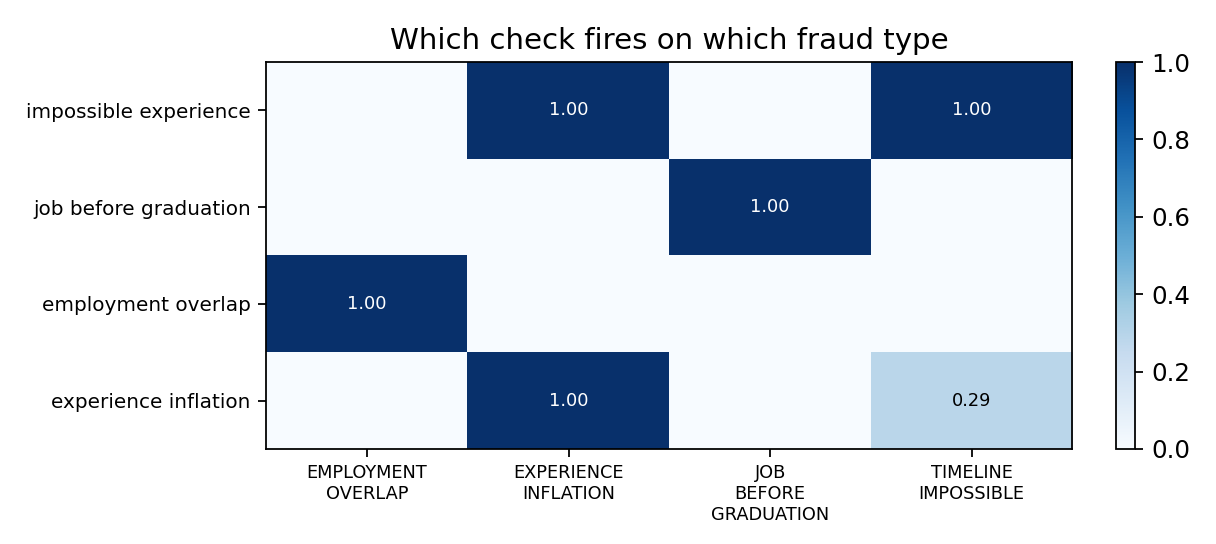
\includegraphics[width=0.82\linewidth]{figures/fig_attribution.png}
\caption{Attribution: fraction of each injected fraud type that triggers each flag
code. Mostly diagonal, with benign cross-firing between impossibility and
inflation.}\label{fig:attribution}
\end{figure}

\begin{table}[t]\centering\small
\caption{Tolerance sweep for the overlap rule ($\theta_o$, months). False-positive
rate on genuine and recall on injected overlaps.}\label{tab:tolerance}
\begin{tabular}{lccccc}
\toprule
$\theta_o$ (months) & 0 & 1 & 3 & 6 & 12 \\
\midrule
FP on genuine & 0.00 & 0.00 & 0.00 & 0.00 & 0.00 \\
Recall on overlap fraud & 1.00 & 1.00 & 1.00 & 1.00 & 1.00 \\
\bottomrule
\end{tabular}
\end{table}

\subsection{Incentive adverse selection}\label{sec:res:incentive}
We simulate a consortium of 12 participants screening 4{,}000 candidates (20\%
fraud, 30\% borderline), over 30 seeds. Under the naive schedule that pays more
for a fraud report, self-interested participants over-label genuine borderline
candidates to farm credits. Table~\ref{tab:incentive} and
Figure~\ref{fig:incentive_ci} report network metrics as the strategic fraction
grows. The naive schedule degrades monotonically and significantly: the network
false-positive rate rises to $0.188$ ($95\%$ CI $[0.173,0.203]$) and precision
falls to $0.60$ at $50\%$ strategic participation. The proposed regime
(outcome-symmetric reward, threshold $t=2$, reputation weighting) holds network
precision at $1.00$ and false positives at $0$ at every level---at the cost of
lower network recall, the correct trade for a legally sensitive shared accusation,
since clear fraud is still caught locally (Section~\ref{sec:res:det}).

\begin{table}[t]\centering\small
\caption{Network false-positive rate vs.\ strategic participation (30 seeds, mean
[95\% CI]).}\label{tab:incentive}
\begin{tabular}{lcc}
\toprule
Strategic \% & Naive FP & Proposed FP \\
\midrule
0  & 0.000 [0.000, 0.000] & \cellcolor{good}0.000 [0.000, 0.000] \\
10 & \cellcolor{bad}0.040 [0.027, 0.054] & \cellcolor{good}0.000 \\
25 & \cellcolor{bad}0.109 [0.090, 0.128] & \cellcolor{good}0.000 \\
40 & \cellcolor{bad}0.160 [0.145, 0.176] & \cellcolor{good}0.000 \\
50 & \cellcolor{bad}0.188 [0.173, 0.203] & \cellcolor{good}0.000 \\
\bottomrule
\end{tabular}
\end{table}

\begin{figure}[t]\centering
\begin{subfigure}{0.49\textwidth}\centering
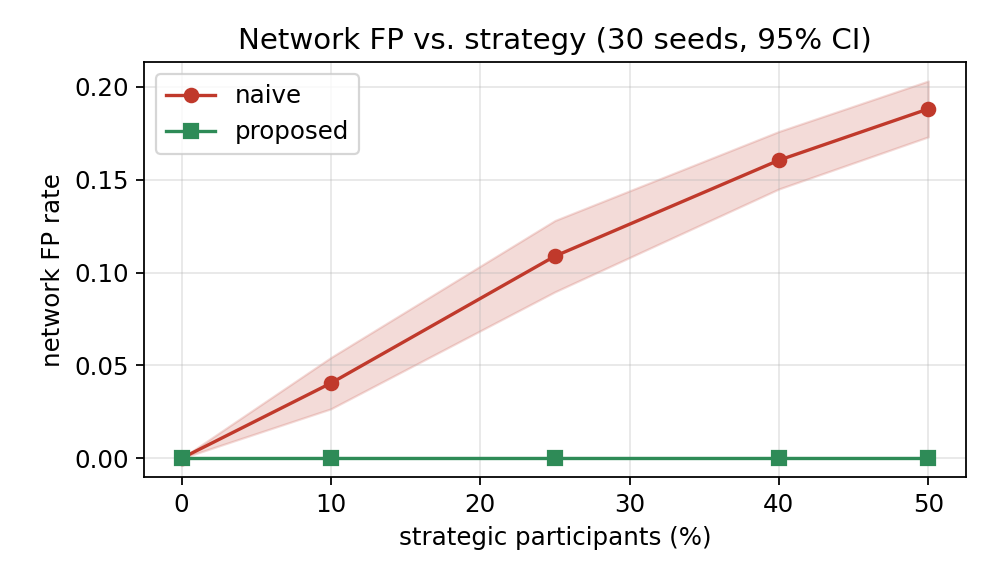
\includegraphics[width=\linewidth]{figures/fig_incentive_ci.png}
\caption{Network FP vs.\ strategy (95\% CI bands).}\label{fig:incentive_ci}
\end{subfigure}\hfill
\begin{subfigure}{0.49\textwidth}\centering
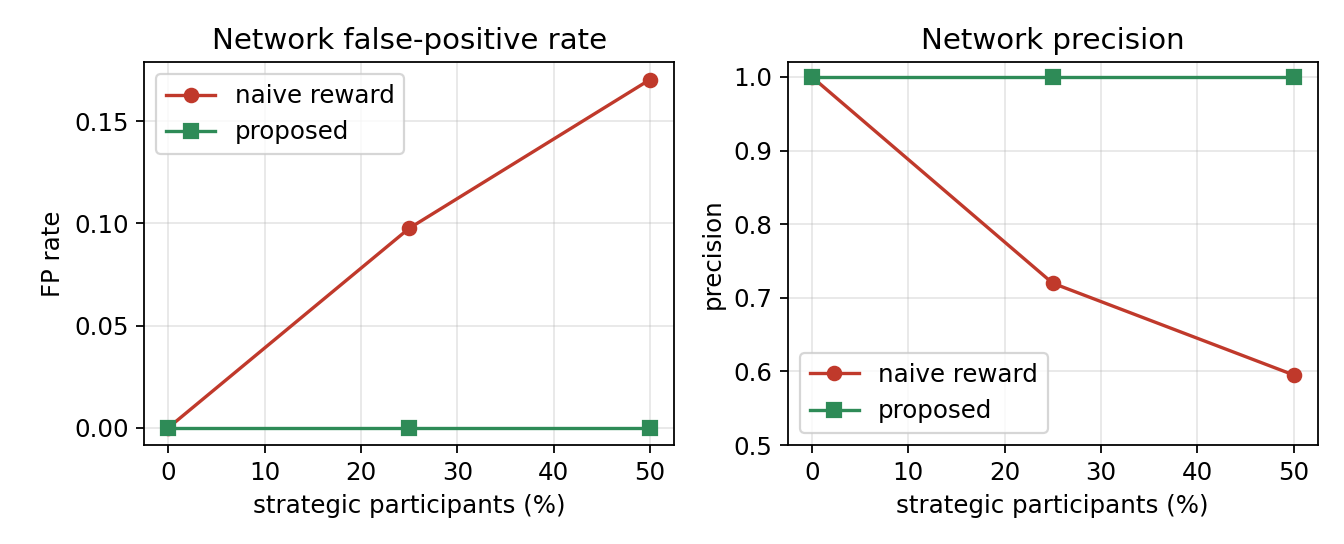
\includegraphics[width=\linewidth]{figures/fig_incentive.png}
\caption{FP (left) and precision (right), single run.}\label{fig:incentive}
\end{subfigure}
\caption{The naive reward corrupts the shared data as strategic behavior rises;
the proposed regime does not.}\label{fig:incentive_both}
\end{figure}

The corroboration threshold $t$ is the knob that buys safety with recall
(Table~\ref{tab:threshold}, Figure~\ref{fig:threshold}). At $t=1$ the proposed
regime already removes farming via outcome symmetry, retaining recall $0.83$; at
$t=2$ recall is $0.41$; beyond $t=3$ the network rarely flags because few
candidates are co-observed by that many organizations at this consortium size.
The takeaway is that $t$ should be set jointly with expected co-observation, which
itself rises with participation (Section~\ref{sec:res:flywheel}).

\begin{table}[t]\centering\small
\caption{Corroboration threshold $t$ vs.\ network recall (proposed regime, 50\%
strategic, 30 seeds). FP is $0$ throughout.}\label{tab:threshold}
\begin{tabular}{lcccc}
\toprule
$t$ & 1 & 2 & 3 & 4 \\
\midrule
Network recall & 0.826 & 0.409 & 0.037 & 0.000 \\
Network FP & 0.000 & 0.000 & 0.000 & 0.000 \\
\bottomrule
\end{tabular}
\end{table}

\begin{figure}[t]\centering
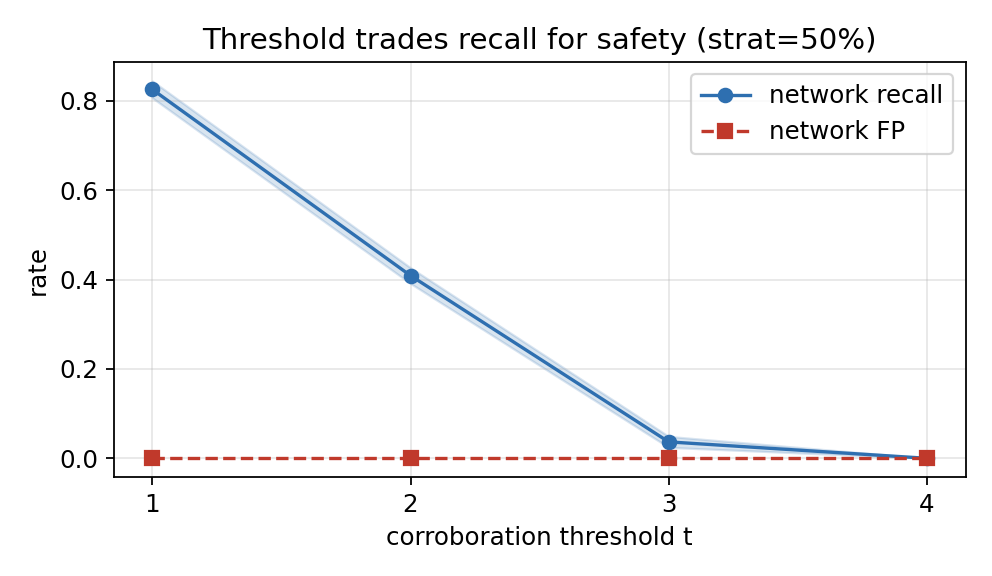
\includegraphics[width=0.6\linewidth]{figures/fig_threshold.png}
\caption{The corroboration threshold trades network recall for safety; FP stays
at $0$.}\label{fig:threshold}
\end{figure}

\subsection{Re-identification}\label{sec:reid}
We populate an identifier universe of 20{,}000 enumerable email+phone pairs, share
4{,}000 as digests, and run $\mathcal{A}_P$. Table~\ref{tab:privacy} gives the
re-identification rate among candidates within the adversary's guess set, and
Figure~\ref{fig:privacy_both} sweeps adversary coverage. Naive hashing leaks in
exact proportion to coverage---an adversary enumerating $c$ of the space recovers
$c$ of the shared set, reaching $100\%$ at full enumeration---because an
employer's own applicant pool \emph{is} such an enumeration. A keyed digest
defeats an outside adversary ($0$) but not a consortium insider ($1.00$), who
holds the key. Only PSI with a corroboration threshold bounds insider leakage to
candidates already co-observed.

\begin{table}[t]\centering\small
\caption{Re-identification rate by sharing construction (universe 20{,}000; shared
4{,}000).}\label{tab:privacy}
\begin{tabular}{lcp{7.0cm}}
\toprule
Construction & Re-id & Notes \\
\midrule
Naive SHA-256(email$\|$phone) & \cellcolor{bad}1.00 & every enumerable candidate recovered exactly \\
Keyed HMAC --- outside adversary & \cellcolor{good}0.00 & cannot compute digests without the key \\
Keyed HMAC --- consortium insider & \cellcolor{bad}1.00 & holds the key $\Rightarrow$ full recovery \\
PSI + disclosure threshold $t$ & bounded & only membership corroborated by $\ge t$ orgs \\
\bottomrule
\end{tabular}
\end{table}

\begin{figure}[t]\centering
\begin{subfigure}{0.49\textwidth}\centering
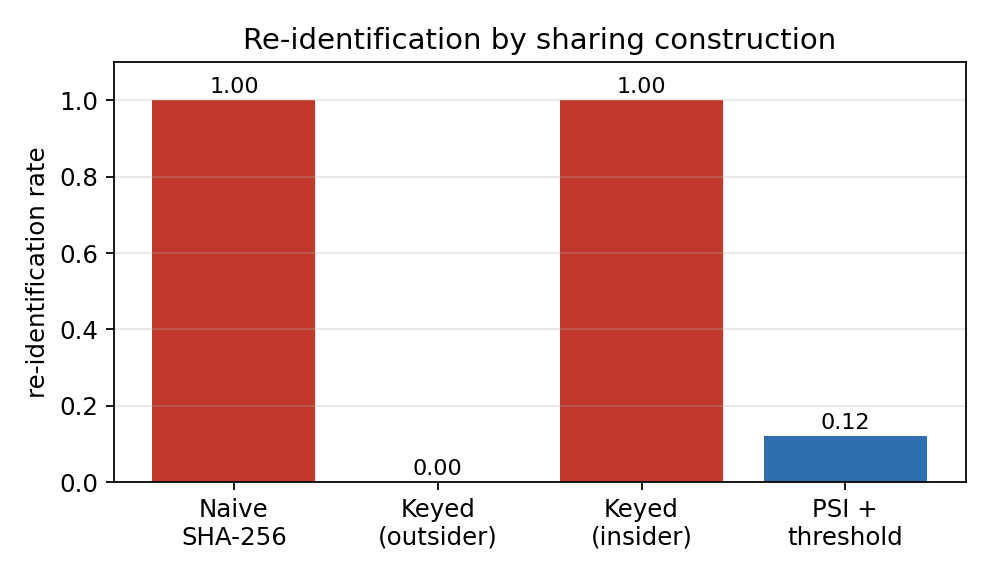
\includegraphics[width=\linewidth]{figures/fig_privacy.png}
\caption{Re-id by construction.}\label{fig:privacy}
\end{subfigure}\hfill
\begin{subfigure}{0.49\textwidth}\centering
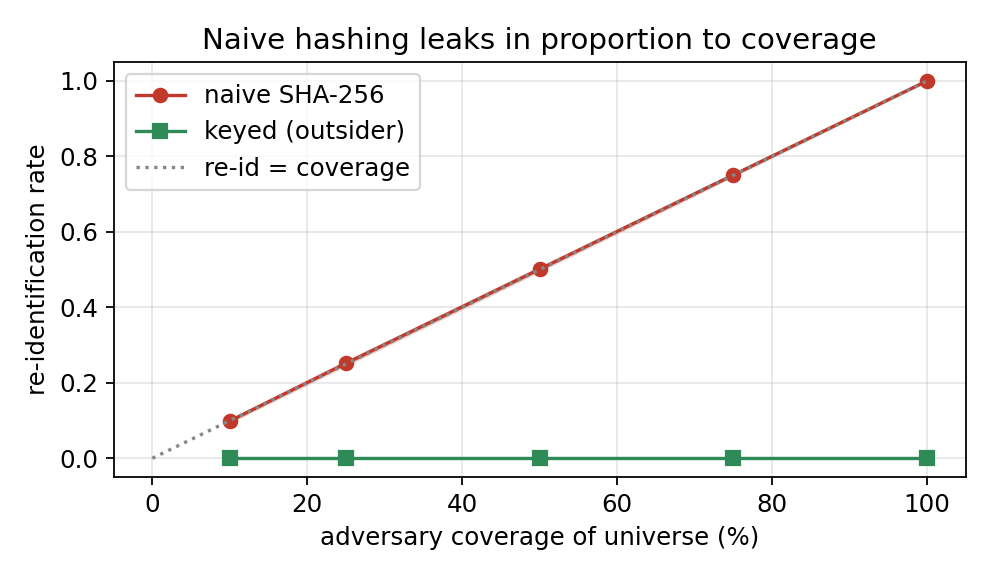
\includegraphics[width=\linewidth]{figures/fig_privacy_coverage.png}
\caption{Naive re-id $=$ adversary coverage.}\label{fig:privacy_coverage}
\end{subfigure}
\caption{Hashing low-entropy identifiers provides no anonymity; re-identification
scales linearly with what the adversary can enumerate.}\label{fig:privacy_both}
\end{figure}

\subsection{AI-fabricated identities}\label{sec:res:agent}
A wholly synthetic identity built by an LLM tends to be internally consistent---so
the deterministic layer cannot catch it---yet, when naively generated, too
regular (round tenures, uniform durations, no gaps). On 1{,}500 fabricated and
1{,}500 genuine trajectories (Table~\ref{tab:agent}), deterministic recall on
fabrications is $0.00$, confirming that well-formed fakes require inferential
signals, while deterministic FP on genuine remains $0.00$. A lightweight
regularity score separates the classes at ROC-AUC $0.90$, with uniformity the
strongest single feature (Figure~\ref{fig:ablation}).

\begin{table}[t]\centering\small
\caption{Detection of AI-fabricated identities ($n=1500$ per class).}\label{tab:agent}
\begin{tabular}{lc}
\toprule
Measure & Value \\
\midrule
Deterministic recall on fabricated & \cellcolor{bad}0.00 \\
Deterministic FP on genuine & 0.00 \\
Regularity-score ROC-AUC (naive fakes) & \cellcolor{good}0.90 \\
Mean regularity (genuine / fabricated) & 0.60 / 0.93 \\
\bottomrule
\end{tabular}
\end{table}

The crucial result is that this inferential defense is \emph{brittle against an
adaptive adversary}. Figure~\ref{fig:sophistication} sweeps a fabrication
``sophistication'' parameter that injects realistic variation (varied start
months, gaps, non-uniform tenures): the regularity detector's AUC collapses from
$0.90$ toward chance by moderate sophistication and below as fabrications acquire
more natural irregularity than our deliberately clean genuine baseline. The honest
reading is that stylometric regularity is a stopgap, not a moat: an adversary who
notices the tell defeats it. This is the central argument for the network layer,
whose signal---recurrence across independent organizations---an adversary cannot
fabricate from within a single application.

\begin{figure}[t]\centering
\begin{subfigure}{0.49\textwidth}\centering
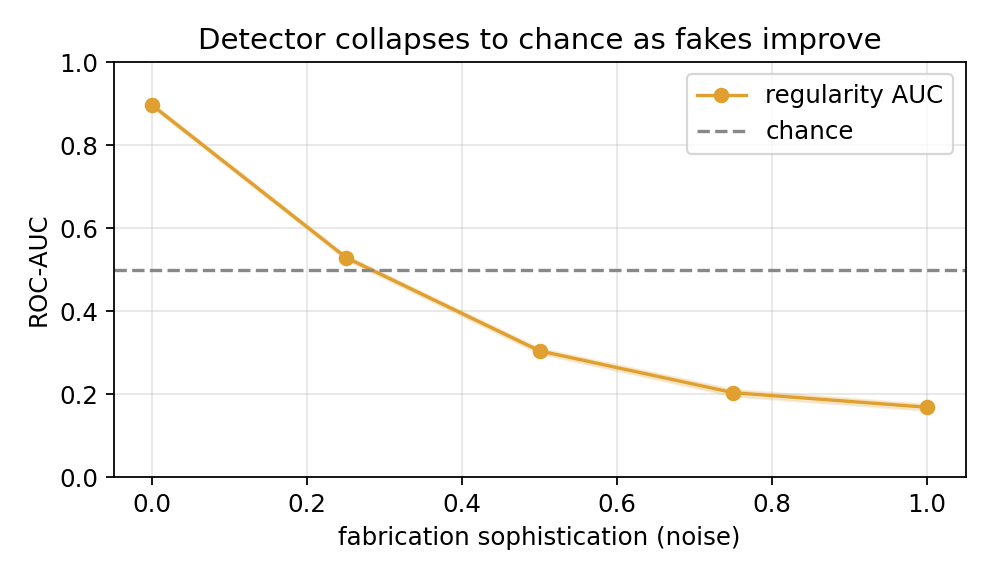
\includegraphics[width=\linewidth]{figures/fig_sophistication.png}
\caption{AUC collapses as fakes improve.}\label{fig:sophistication}
\end{subfigure}\hfill
\begin{subfigure}{0.49\textwidth}\centering
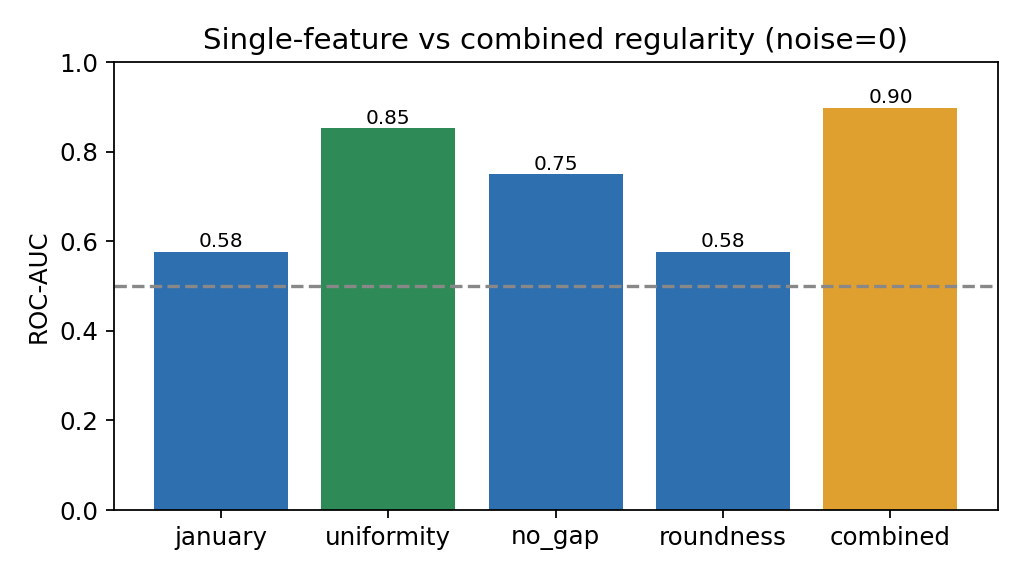
\includegraphics[width=\linewidth]{figures/fig_ablation.png}
\caption{Single-feature vs combined (naive fakes).}\label{fig:ablation}
\end{subfigure}
\caption{The regularity detector works on naive fabrications (left, noise $0$) but
degrades to chance against an adaptive adversary; uniformity is the strongest
single feature (right).}\label{fig:agent_both}
\end{figure}

\subsection{The contributory-network flywheel}\label{sec:res:flywheel}
The network's value grows with participation. We simulate repeat fraudsters who
apply to several organizations; a repeat application is caught network-wide when
the actor has already been reported by $\ge t$ in-network organizations.
Figure~\ref{fig:flywheel} plots the repeat-fraud catch rate against the fraction
of organizations on the network. The curve is convex and steepening: at $25\%$
participation only $6\%$ of repeat fraud is caught, but at $75\%$ it is $46\%$ and
at full participation $67\%$. This is the contributory moat made quantitative, and
it explains why the threshold $t$ and participation must be set together---higher
participation raises co-observation, which makes a given $t$ less costly in recall.

\begin{figure}[t]\centering
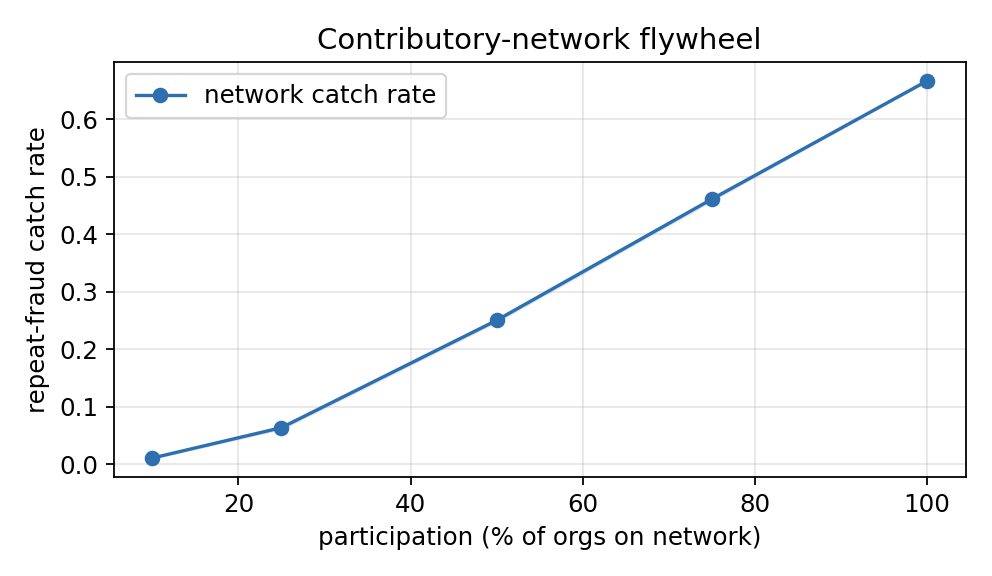
\includegraphics[width=0.6\linewidth]{figures/fig_flywheel.png}
\caption{Repeat-fraud catch rate rises with the fraction of organizations on the
network (20 seeds, 95\% CI).}\label{fig:flywheel}
\end{figure}

\subsection{Fraud-ring detection}\label{sec:res:ring}
A single actor may apply under many synthetic identities. If those identities
share a secondary identifier (a reused phone, device, or reference), the network
links them. Figure~\ref{fig:fraud_ring} plots detection rate against the number of
identities $k$ a ring uses: detection rises from $0$ at $k=1$ (a lone identity is
indistinguishable) to $0.49$ at $k=2$, $0.78$ at $k=3$, and $0.99$ at $k=6$. The
mechanism that makes a ring effective---reusing infrastructure across many
identities---is exactly what makes it detectable once organizations share.

\begin{figure}[t]\centering
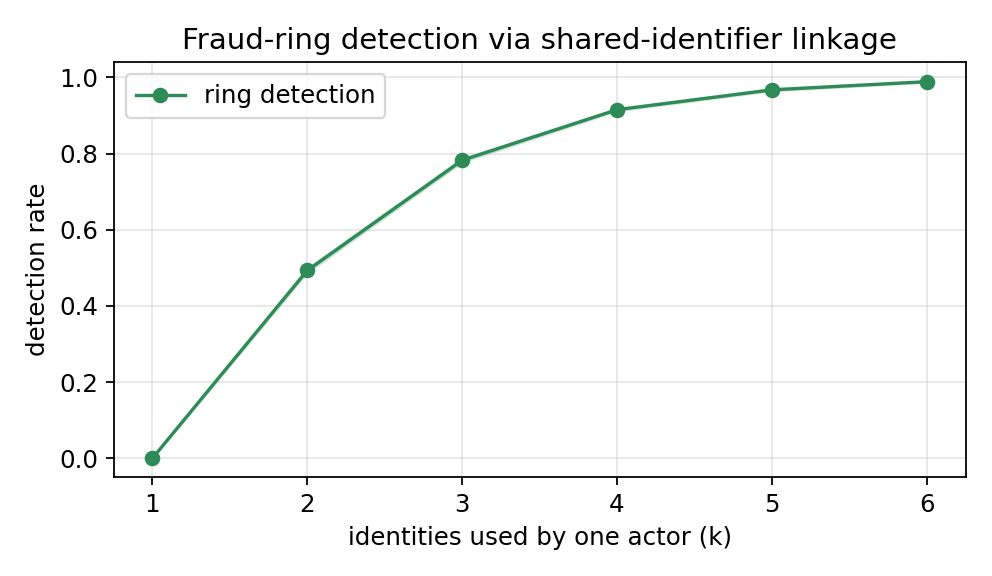
\includegraphics[width=0.6\linewidth]{figures/fig_fraud_ring.png}
\caption{Fraud-ring detection via shared-identifier linkage rises with the number
of identities the ring uses (20 seeds, 95\% CI).}\label{fig:fraud_ring}
\end{figure}

\subsection{Contribution economics}\label{sec:res:econ}
Finally, the incentive only works if contributing is cheaper than not. Under a
simple model where contributed profiles earn credits that offset check costs,
Figure~\ref{fig:economics} and Table~\ref{tab:econ} show effective price per check
falling from \$0.75 to \$0.375 as the contribution ratio rises to parity---a
$50\%$ saving for an organization that contributes as much as it consumes. This is
the financial counterpart to the corrected incentive: members are rewarded for
\emph{participation}, symmetrically across outcomes, rather than for producing
fraud verdicts.

\begin{table}[t]\centering\small
\caption{Contribution-credit economics (illustrative model).}\label{tab:econ}
\begin{tabular}{lccccc}
\toprule
Contribution ratio & 0\% & 25\% & 50\% & 75\% & 100\% \\
\midrule
Effective \$/check & 0.750 & 0.656 & 0.562 & 0.469 & 0.375 \\
Saving & 0\% & 12.5\% & 25\% & 37.5\% & 50\% \\
\bottomrule
\end{tabular}
\end{table}

\begin{figure}[t]\centering
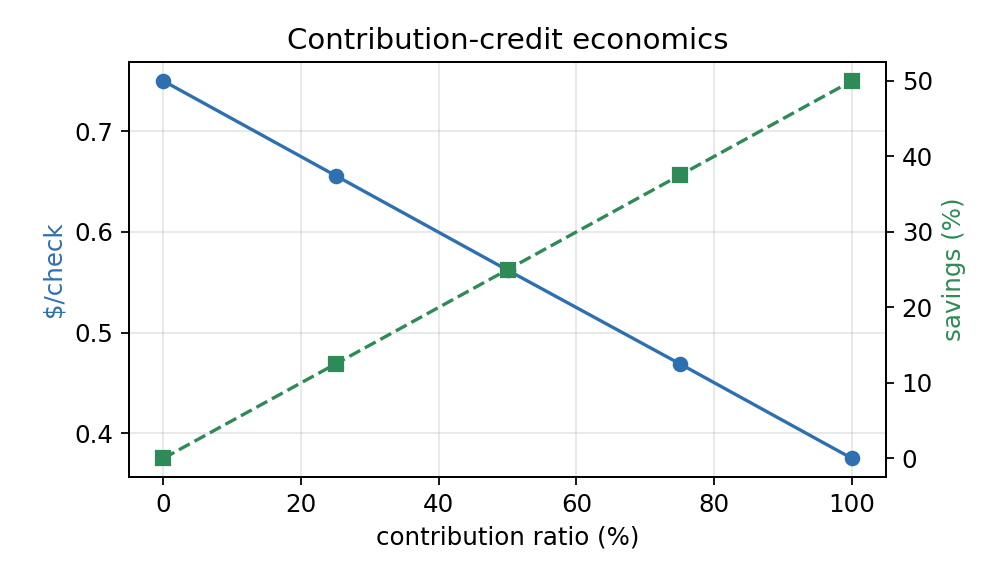
\includegraphics[width=0.6\linewidth]{figures/fig_economics.png}
\caption{Effective price per check and savings vs.\ contribution
ratio.}\label{fig:economics}
\end{figure}

\section{Related Systems and Positioning}\label{sec:positioning}
TruthHire occupies a position no existing system holds. Background-screening
vendors verify against authoritative records; payroll-network services confirm
employment for enrolled employers; national fraud consortia share signals within
a single regulated industry; and the academic literature contributes detection
models and private-set-intersection protocols in isolation. Table~\ref{tab:systems}
contrasts the axes that matter: the \emph{evidence model} (authoritative
verification versus inference from claims), \emph{cross-organization} memory,
\emph{privacy} method, \emph{incentive} design, and whether the system treats
\emph{experience-timeline} fraud as a first-class target.

\begin{table}[t]\centering\small
\caption{Positioning against representative systems and lines of work.}\label{tab:systems}
\begin{tabular}{p{2.6cm}p{2.2cm}cp{2.0cm}p{2.0cm}c}
\toprule
System / line & Evidence model & Cross-org & Privacy method & Incentive & Timeline focus\\
\midrule
HireRight, Checkr, Sterling & verification & no & N/A & fee-for-service & no\\
The Work Number & payroll records & enrolled only & contractual & employer supply & partial\\
Cifas / national consortia & member reports & yes (finance) & membership rules & regulatory & no\\
Verisk ClaimSearch & contributory & yes (insurance) & contractual & loss-ratio & no\\
Federated fraud ML~\cite{starlit2024} & model sharing & yes & federated learning & none specified & no\\
Multi-party PSI~\cite{otpsi2026} & set membership & yes & PSI & none specified & no\\
\textbf{TruthHire (this work)} & deterministic + inference + network & yes (hiring) & threshold PSI & outcome-symmetric & \textbf{yes}\\
\bottomrule
\end{tabular}
\end{table}

The synthesis is the contribution. Verification is stronger evidence than
inference but is unavailable for most of the world's employers and roles; the
deterministic layer recovers much of verification's reliability for the specific
case of \emph{internal} timeline consistency without any external lookup. The
consortium model is proven in finance but has never been paired with an
incentive design that resists the fraud-reporting adverse selection we identify,
nor adapted to the FCRA/GDPR posture that hiring demands.

\section{Deployment and Integration Architecture}\label{sec:deploy}
The system is delivered as an API that an applicant-tracking system or careers
portal integrates once. Table~\ref{tab:endpoints} lists the surface. The design
keeps the latency-sensitive path (the deterministic layer) free of any external
call, so a synchronous verdict returns in milliseconds; inferential and network
signals run asynchronously and are delivered by webhook, which also matches their
advisory status---a human reviewer, not the request, consumes them.

\begin{table}[t]\centering\small
\caption{API surface. The dispute and audit endpoints are required by the
governance posture of Section~\ref{sec:legal}.}\label{tab:endpoints}
\begin{tabular}{lll}
\toprule
Endpoint & Method & Purpose\\
\midrule
\code{/verify} & POST & deterministic + (async) inferential analysis\\
\code{/contribute} & POST & add an audited signal record to the network\\
\code{/flags/lookup} & POST & threshold-PSI membership query\\
\code{/dispute} & POST & candidate-initiated reinvestigation request\\
\code{/audit/\{check\}} & GET & explanation and provenance for a decision\\
\code{/candidate/\{id\}} & DELETE & erasure (GDPR right to be forgotten)\\
\bottomrule
\end{tabular}
\end{table}

A realistic latency budget (Table~\ref{tab:latency}) makes the layering concrete:
the deterministic layer is essentially free, while any layer that touches an
external service or a PSI round dominates and therefore belongs off the
synchronous path. Audit logging---storing which rule fired and on what input---is
cheap and is what makes the dispute endpoint and FCRA reinvestigation feasible.

\begin{table}[t]\centering\small
\caption{Illustrative latency budget by layer.}\label{tab:latency}
\begin{tabular}{lll}
\toprule
Layer & Typical latency & Path\\
\midrule
Deterministic timeline & $<5$ ms & synchronous\\
Inferential (per external signal) & $0.2$--$2$ s & asynchronous\\
Threshold-PSI network query & $0.1$--$1$ s & asynchronous\\
\bottomrule
\end{tabular}
\end{table}

\section{A Threshold-PSI Sharing Protocol}\label{sec:protocol}
We sketch the sharing protocol and its leakage. Each organization holds a set of
reported-candidate identifiers. A query asks: is this candidate present in at
least $t$ organizations' sets? The protocol must answer that and nothing
more---in particular it must not reveal \emph{which} organizations, nor any
non-matching identifiers, nor allow an enumerating adversary to test arbitrary
guesses offline. Over-threshold multi-party PSI provides exactly this
primitive~\cite{otpsi2026}; Algorithm~4 states the wrapper.

\begin{algbox}{Algorithm 4: threshold-PSI network query}
\ttfamily\small
\textbf{setup} each org $o$ commits its reported set $R_o$ under MPC-PSI protocol $\Pi$\\
\textbf{query}$(\mathrm{id}, t)$:\\
\hspace*{1.2em}$c \leftarrow \Pi.\textsc{OverThresholdCount}(\mathrm{id}, t)$\ \ // \#orgs with id, only if $\ge t$\\
\hspace*{1.2em}\textbf{if} $c \ge t$:\ \textbf{return} \code{FLAG}$(c)$;\ \textbf{else} \textbf{return} \code{NONE}\\
\textbf{leakage} to a single party: membership bit and count, only for $c\ge t$;\\
\hspace*{1.2em}nothing for $c<t$; no identities; no per-org attribution
\end{algbox}

Table~\ref{tab:leakage} compares constructions by what each leaks and at what
cost. The progression is monotone: the cheaper the construction, the more it
leaks. Naive publication leaks everything enumerable for free; a network pepper
shifts the leak from outsiders to insiders; threshold PSI pays computation to
leak only corroborated membership. The design recommendation follows the threat
model rather than the benchmark: because a consortium insider is in scope, only
the threshold-PSI row satisfies goal~G2 of Property~\ref{prop:goals}.

\begin{table}[t]\centering\small
\caption{Leakage and cost by sharing construction.}\label{tab:leakage}
\begin{tabular}{lp{4.0cm}p{4.6cm}}
\toprule
Construction & Leaks to & Cost\\
\midrule
Publish SHA-256 & anyone who can enumerate & negligible\\
Keyed HMAC & any key-holder (every insider) & negligible\\
PSI (pairwise) & matching set to both parties & moderate (crypto)\\
\rowcolor{good} Threshold PSI & corroborated membership only & higher (MPC)\\
\bottomrule
\end{tabular}
\end{table}

\section{Worked Scenarios}\label{sec:scenarios}
Three candidates illustrate how the layers divide labor and where governance
intervenes.

\paragraph{Scenario 1: the impossible junior.} A 24-year-old claims 15 years of
experience across three roles. The deterministic layer fires
\code{TIMELINE\_IMPOSSIBLE} ($y=15 > a-18=6$) and \code{EXPERIENCE\_INFLATION},
returning a high score with an explainable reason in milliseconds and no external
data. This is the engine's home ground: explainable, certain, and cheap.

\paragraph{Scenario 2: the privacy-minimal senior.} A genuine 48-year-old
principal engineer has a sparse digital footprint, no public GitHub, and a thin
search presence. The deterministic layer is silent (her timeline is consistent).
The inferential layer would raise low-confidence signals (\code{NO\_WEB\_PRESENCE},
\code{GITHUB\_INACTIVE})---and this is exactly the false-positive risk that the
advisory, human-in-the-loop posture exists to absorb. Under our design these
signals never auto-reject; they surface to a reviewer who, seeing a coherent
senior r\'esum\'e, dismisses them. Under a naive auto-reject design she is wrongly
filtered out. Scenario 2 is the paper's ethical core in miniature.

\paragraph{Scenario 3: the distributed ring.} One actor applies to three member
organizations under three identities that share a reused phone number. No single
organization sees anything amiss. The threshold-PSI query
(Algorithm~4, $t=2$) links the identities via the shared identifier once two
organizations have reported, and the ring surfaces---precisely the
cross-organization memory that no isolated screen can provide
(Section~\ref{sec:res:ring}).

\section{Governance, Audit, and Dispute Workflow}\label{sec:governance}
Because the system can influence employment outcomes, governance is not optional
tooling but a core component. Table~\ref{tab:obligations} maps each major legal
obligation onto the concrete feature that discharges it, demonstrating that the
architecture was derived from the constraints rather than retrofitted to them.

\begin{table}[t]\centering\small
\caption{Mapping legal obligations to system features.}\label{tab:obligations}
\begin{tabular}{p{3.4cm}p{3.0cm}p{6.2cm}}
\toprule
Obligation & Source & Feature\\
\midrule
Maximum-possible accuracy & FCRA & deterministic core; evidence-gated network; reputation weighting\\
Disclosure \& authorization & FCRA & consent capture at application; per-portal notices\\
Adverse-action procedure & FCRA & advisory-only outputs; human-in-the-loop gate\\
Dispute \& reinvestigation & FCRA & \code{/dispute} endpoint; audit log of every flag\\
Lawful basis; Art.\ 22 & GDPR & no solely-automated significant decision; human review\\
Right to erasure & GDPR & \code{/candidate/\{id\}} delete; retention limits\\
Data minimization & GDPR & signal records carry hashes + flags, never raw PII\\
\bottomrule
\end{tabular}
\end{table}

The dispute lifecycle is concrete. A candidate who is told they were
adversely affected may invoke reinvestigation; the system retrieves the audit
record for the decision (which rule fired on which input), re-runs the
deterministic layer deterministically (the same input yields the same result),
and, for network signals, re-checks corroboration. Because the deterministic
layer is explainable by construction, a dispute resolves to a human-legible
statement---``flagged because claimed experience exceeds the maximum possible
given the stated age''---rather than to an opaque model score. This is the
operational reason the paper privileges the deterministic layer: it is the only
layer whose decisions can be defended, line by line, in a reinvestigation.

\section{Mechanism-Design Analysis}\label{sec:mechanism}
We now argue more formally why the incentive correction works. Consider a
participant deciding how to label a borderline genuine candidate. Let the reward
for a report be $\rho(\ell, o)$ where $\ell$ is the submitted label and $o$ the
eventual audited outcome, and let $\Delta = \rho(\text{fraud}, \cdot) -
\rho(\text{legit}, \cdot)$ be the schedule's fraud premium. Under the naive
schedule $\Delta > 0$ regardless of $o$, so for a borderline case where the
participant is indifferent on the merits, reporting \emph{fraud} strictly
dominates reporting \emph{legit}: it earns $\Delta$ more at no cost. Farming is a
best response, and its prevalence scales with the strategic fraction---exactly the
monotone degradation observed in Table~\ref{tab:incentive}.

\begin{property}[Farming-proofness under symmetry]\label{prop:sym}
If the reward depends only on whether the report matches the audited outcome---
$\rho(\ell,o)=\beta\,\mathbf{1}[\ell=o]$ for a constant $\beta$, so $\Delta=0$ in
expectation over a borderline case---then truthful reporting weakly dominates
farming, and strictly dominates it whenever the audited outcome is more likely
legitimate than not.
\end{property}

\noindent Outcome symmetry sets $\Delta=0$ and removes the farming gradient;
evidence gating raises the cost of a fraud report (it must carry qualifying
evidence); and reputation weighting (Algorithm~3) imposes a dynamic penalty,
multiplying a participant's influence by its historical accuracy so that a farmer's
reports decay toward zero weight. Table~\ref{tab:schedules} summarizes the
qualitative effect of each schedule on the two quantities that matter, data
quality and participation; the simulations of Section~\ref{sec:res:incentive}
instantiate the top and bottom rows.

\begin{table}[t]\centering\small
\caption{Incentive schedules and their qualitative effects.}\label{tab:schedules}
\begin{tabular}{lcc}
\toprule
Schedule & Data quality & Participation\\
\midrule
\rowcolor{bad} Fraud-weighted (naive) & degrades with strategy & high\\
Outcome-symmetric & preserved & high\\
\rowcolor{good} Symmetric + evidence + reputation & preserved under strategy & high\\
No reward & preserved & low (cold-start fails)\\
\bottomrule
\end{tabular}
\end{table}

The design therefore threads a needle the financial-consortium literature does not
face: it must reward contribution strongly enough to bootstrap participation
(the bottom row fails the cold start) while attaching the reward to verified
information rather than to a verdict the contributor itself supplies (the top row
fails accuracy). The middle rows are the feasible region.

\section{Alternative Designs Considered}\label{sec:alternatives}
Several plausible architectures were rejected; stating why sharpens the design.
Table~\ref{tab:alternatives} summarizes the trade.

\begin{table}[t]\centering\small
\caption{Alternatives considered and why the chosen design is preferred.}\label{tab:alternatives}
\begin{tabular}{p{3.3cm}p{5.0cm}p{4.4cm}}
\toprule
Alternative & Why attractive & Why rejected\\
\midrule
Central trusted clearinghouse & simple matching, low latency & single point of breach; concentrates derogatory PII; weak GDPR posture\\
ML-only detection & captures subtle patterns & opaque; undefendable in dispute; high FP on atypical genuine candidates\\
Reputation only (no threshold) & cheap; no MPC & a single confident farmer still injects false flags\\
Blockchain ledger of flags & tamper-evidence; decentralization & immutable derogatory records conflict with erasure and dispute rights\\
\rowcolor{good} Deterministic-first + threshold-PSI + symmetric incentives (this work) & explainable, minimally leaky, gaming-resistant & higher cryptographic cost (acceptable off the synchronous path)\\
\bottomrule
\end{tabular}
\end{table}

Two rejections are worth emphasizing. A central clearinghouse is the obvious
engineering choice and the wrong privacy choice: it converts a distributed,
threshold-gated leakage profile into a single honeypot of derogatory personal
data, precisely what GDPR's data-minimization principle counsels against. And an
immutable ledger, attractive for tamper-evidence, is incompatible with the right
to erasure and with reinvestigation: a flag that later proves wrong must be
removable, and a candidate's successful dispute must actually delete the
accusation, not merely append a correction the next employer may never read.

\section{Sensitivity Analysis and Threats to Validity}\label{sec:validity}

\paragraph{Construct validity.} Our genuine population is, in the controlled
experiments, synthetic and deliberately clean; it therefore \emph{understates} the
deterministic layer's false-positive rate, which on real atypical careers will be
positive. We are explicit that the headline external measurement---FP on
KARRIEREWEGE---is future work, and our harness is built to run it unchanged.

\paragraph{Internal validity.} The incentive and flywheel results are simulations
with stated generative assumptions (consortium size, fraud prior, co-observation).
We report $95\%$ confidence intervals over many seeds and provide sweeps over the
key parameters (threshold, strategy, participation) so the trends, not single
points, carry the argument. The qualitative conclusions---naive reward corrupts
the network; thresholding trades recall for safety; participation compounds
value---are robust across the swept ranges.

\paragraph{The agent detector.} The AUC-versus-sophistication result deliberately
exposes a limitation: against an adaptive adversary the stylometric detector
fails, and the sub-chance region reflects our clean baseline rather than
``reverse'' detection power. We present it not as a capability but as the empirical
case for relying on cross-organization recurrence over single-application
stylometry.

\paragraph{External validity.} Re-identification is computed on a synthetic
identifier universe, but the result is structural---low-entropy enumerable
identifiers cannot be anonymized by hashing---and matches the cryptographic
literature~\cite{cook2019,otpsi2026}. The economics model is illustrative and not
a pricing recommendation.

\section{Discussion}\label{sec:discuss}
Three themes recur. First, \emph{explainability is a safety feature, not a
nicety}: the deterministic layer's transparency is what makes dispute,
reinvestigation, and audit feasible under FCRA. Second, \emph{the network's
strength is also its danger}: cross-employer memory is the unique value, but a
false signal in that memory is repeated and amplified, which is why the privacy,
incentive, and governance designs are not separable from the detection design.
Third, \emph{incentives must reward information, not verdicts}: the single most
consequential design error we identify is paying for fraud findings, and it is
also the cheapest to fix.

\section{Ethics and Responsible Disclosure}\label{sec:ethics}
The dominant risk is not missed fraud but \emph{wrongful suspicion}: a false
positive can quietly cost a real person a job, and a shared false positive can do
so repeatedly and invisibly. This motivates the advisory-only stance, the dispute
mechanism, the false-positive-cost metric, and the evidence-gated network. The
work is dual-use---a detector and a generator co-evolve, as
Section~\ref{sec:res:agent} shows---and the inferential signals risk encoding bias
against candidates with non-standard or low-digital-footprint histories,
including along national and cultural lines. We therefore (a) keep inferential and
network signals advisory; (b) prioritize the explainable deterministic layer; (c)
release the implementation openly for scrutiny before any commercial use; and (d)
defer commercial operation, which triggers the heaviest regulatory duties. We do
not claim the deterministic layer is novel in isolation; its value is as the
explainable backbone of an integrated, shared, regulation-aware system.

\section{Limitations and Research Agenda}\label{sec:agenda}
The central open item is empirical and external: a multi-organization study with
consenting partners to validate the flywheel at scale, and a measurement of the
deterministic and inferential false-positive rates on real, atypical KARRIEREWEGE
trajectories and across demographic and cultural cohorts (a fairness audit). On
the cryptographic side, a formal security proof and a performance evaluation of
the chosen threshold-PSI protocol are needed. On the detection side, richer
inferential features and their adaptive-adversary robustness deserve study, as
does integration with real LLM-generated r\'esum\'es rather than our stylized
fabricator. None of these changes the framework; they instantiate and stress it.

\section{Conclusion}\label{sec:conclusion}
Employment-experience fraud is a coordination failure: defenders act alone while
attackers reuse fabricated identities across them. Other industries closed this
gap with privacy-preserving contributory networks, but doing so for hiring
requires jointly solving detection, re-identification-resistant sharing,
contribution incentives, and regulatory constraints---problems previously studied
apart. We framed that integration; gave a deterministic, explainable detection
core; demonstrated, with confidence intervals and parameter sweeps, why two common
shortcuts (hash-as-anonymization and fraud-weighted rewards) fail and how to fix
them; quantified the contributory flywheel and fraud-ring detection; and grounded
every decision in FCRA and GDPR constraints. The next step is an open,
multi-organization study to validate the network effect and to measure, above
all, the cost the system imposes on the innocent.

\bibliographystyle{plain}
\bibliography{references}

\appendix
\section{Notation}\label{app:notation}
\begin{table}[h]\centering\small
\begin{tabular}{ll}
\toprule
Symbol & Meaning \\
\midrule
$a,g,y$ & age, graduation year, total claimed years \\
$J=\{(s_i,e_i,\tau_i)\}$ & job intervals (start, end, type) \\
$\theta_o,\theta_y$ & overlap (months) and inflation (years) tolerances \\
$t$ & corroboration / disclosure threshold \\
$\mathrm{rep}[p]$ & reputation weight of participant $p$ \\
$\mathcal{A}_C,\mathcal{A}_P,\mathcal{A}_I$ & candidate, privacy, incentive adversaries \\
\bottomrule
\end{tabular}
\end{table}

\section{Flag reference}\label{app:flags}
\begin{table}[h]\centering\small
\begin{tabular}{llc}
\toprule
Flag code & Severity & Points \\
\midrule
\code{TIMELINE\_IMPOSSIBLE} & Critical & +50 \\
\code{JOB\_BEFORE\_GRADUATION} & Critical & +40 \\
\code{EMPLOYMENT\_OVERLAP} & High & +25 each \\
\code{EXPERIENCE\_INFLATION} & High & +25 \\
\code{NETWORK\_FLAG}$(c)$ & High/Critical & threshold-gated \\
\bottomrule
\end{tabular}
\end{table}

\section{Hyperparameters}\label{app:hyper}
\begin{table}[h]\centering\small
\begin{tabular}{lll}
\toprule
Experiment & Parameter & Value \\
\midrule
Deterministic & population $n$ / fraud rate & 3000 / 0.5 \\
Deterministic & $\theta_o$ / $\theta_y$ & 3 mo / 1 yr \\
Incentive & participants / candidates & 12 / 4000 \\
Incentive & fraud prior / borderline & 0.20 / 0.30 \\
Incentive & threshold $t$ (proposed) & 2 \\
Incentive & seeds & 30 \\
Privacy & universe / shared & 20000 / 4000 \\
Agent & per class $n$ / seeds & 1500 / 10 \\
Flywheel & orgs / apps-per-actor & 50 / 4 \\
All & master seed & 20260612 \\
\bottomrule
\end{tabular}
\end{table}

\section{Reproducibility checklist}\label{app:repro}
The released repository~\cite{truthhirecode} contains: the deterministic engine
and unit tests; the seed tables and deterministic dataset generator with a
provenance hash; the fraud-injection, evaluation, incentive, privacy, agent,
network, and sweep modules; the figure-generation scripts; and a download script
for the external corpora. Each command in the repository README reproduces a named
table or figure in this paper from the same master seed.

\section{Full experimental results}\label{app:full}
All values are means over the stated number of seeds with 95\% confidence intervals where applicable; they are emitted directly from \code{results/study.json} in the released harness.
\begin{table}[h]\centering\small\caption{Incentive study: network FP, precision, recall vs.\ strategic participation (30 seeds).}\label{tab:app:inc}
\begin{tabular}{lllll}\toprule Strat. & Regime & FP & Precision & Recall\\\midrule
0\% & naive & 0.000 [0.000, 0.000] & 1.000 [1.000, 1.000] & 1.000 [1.000, 1.000]\\
0\% & proposed & 0.000 [0.000, 0.000] & 1.000 [1.000, 1.000] & 0.669 [0.663, 0.674]\\
10\% & naive & 0.040 [0.027, 0.054] & 0.875 [0.838, 0.911] & 1.000 [1.000, 1.000]\\
10\% & proposed & 0.000 [0.000, 0.000] & 1.000 [1.000, 1.000] & 0.610 [0.591, 0.629]\\
25\% & naive & 0.109 [0.090, 0.128] & 0.713 [0.674, 0.752] & 1.000 [1.000, 1.000]\\
25\% & proposed & 0.000 [0.000, 0.000] & 1.000 [1.000, 1.000] & 0.513 [0.488, 0.539]\\
40\% & naive & 0.160 [0.145, 0.176] & 0.617 [0.591, 0.643] & 1.000 [1.000, 1.000]\\
40\% & proposed & 0.000 [0.000, 0.000] & 1.000 [1.000, 1.000] & 0.448 [0.428, 0.467]\\
50\% & naive & 0.188 [0.173, 0.203] & 0.577 [0.557, 0.597] & 1.000 [1.000, 1.000]\\
50\% & proposed & 0.000 [0.000, 0.000] & 1.000 [1.000, 1.000] & 0.409 [0.391, 0.427]\\
\bottomrule\end{tabular}\end{table}
\begin{table}[h]\centering\small\caption{Threshold sweep (proposed regime, 50\% strategic, 30 seeds).}\label{tab:app:thr}
\begin{tabular}{lll}\toprule $t$ & FP & Recall\\\midrule
1 & 0.000 [0.000, 0.000] & 0.826 [0.807, 0.845]\\
2 & 0.000 [0.000, 0.000] & 0.409 [0.391, 0.427]\\
3 & 0.000 [0.000, 0.000] & 0.037 [0.024, 0.049]\\
4 & 0.000 [0.000, 0.000] & 0.000 [0.000, 0.000]\\
\bottomrule\end{tabular}\end{table}
\begin{table}[h]\centering\small\caption{Re-identification vs.\ adversary coverage (10 seeds).}\label{tab:app:priv}
\begin{tabular}{lll}\toprule Coverage & Naive re-id & Keyed (outsider)\\\midrule
10\% & 0.099 [0.095, 0.102] & 0.000 [0.000, 0.000]\\
25\% & 0.252 [0.247, 0.257] & 0.000 [0.000, 0.000]\\
50\% & 0.501 [0.496, 0.506] & 0.000 [0.000, 0.000]\\
75\% & 0.751 [0.748, 0.754] & 0.000 [0.000, 0.000]\\
100\% & 1.000 [1.000, 1.000] & 0.000 [0.000, 0.000]\\
\bottomrule\end{tabular}\end{table}
\begin{table}[h]\centering\small\caption{Regularity-detector AUC vs.\ fabrication sophistication (10 seeds).}\label{tab:app:soph}
\begin{tabular}{ll}\toprule Noise & ROC-AUC\\\midrule
0.0 & 0.896 [0.891, 0.901]\\
0.25 & 0.529 [0.524, 0.534]\\
0.5 & 0.304 [0.298, 0.311]\\
0.75 & 0.203 [0.195, 0.212]\\
1.0 & 0.168 [0.161, 0.176]\\
\bottomrule\end{tabular}\end{table}
\begin{table}[h]\centering\small\caption{Single-feature vs combined regularity AUC (noise $=0$).}\label{tab:app:abl}
\begin{tabular}{ll}\toprule Feature & ROC-AUC\\\midrule
january & 0.577\\
uniformity & 0.853\\
no gap & 0.750\\
roundness & 0.577\\
combined & 0.899\\
\bottomrule\end{tabular}\end{table}
\begin{table}[h]\centering\small\caption{Network flywheel and fraud-ring detection (20 seeds).}\label{tab:app:net}
\begin{tabular}{lll}\toprule Participation & Catch rate & \\\midrule
10\% & 0.011 [0.010, 0.011] & \\
25\% & 0.064 [0.062, 0.065] & \\
50\% & 0.250 [0.248, 0.252] & \\
75\% & 0.461 [0.459, 0.463] & \\
100\% & 0.667 [0.667, 0.667] & \\
\midrule Identities $k$ & Ring detection & \\\midrule
1 & 0.000 [0.000, 0.000] & \\
2 & 0.493 [0.488, 0.499] & \\
3 & 0.783 [0.777, 0.788] & \\
4 & 0.915 [0.912, 0.918] & \\
5 & 0.967 [0.965, 0.970] & \\
6 & 0.989 [0.987, 0.991] & \\
\bottomrule\end{tabular}\end{table}

\section{Reproduction map}\label{app:repromap}
Each result in this paper is regenerated by a single command in the released
harness~\cite{truthhirecode} from master seed \texttt{20260612}.

\begin{table}[h]\centering\small
\begin{tabular}{lll}
\toprule
Artifact & Module & Command\\
\midrule
Table~\ref{tab:det} & \code{evaluate} & \code{run\_experiment}\\
Fig.~\ref{fig:attribution}, Table~\ref{tab:tolerance} & \code{sweeps} & \code{make\_study\_figures}\\
Tables~\ref{tab:incentive},~\ref{tab:threshold}, Figs.~\ref{fig:incentive_ci},~\ref{fig:threshold} & \code{sim\_incentive}, \code{sweeps} & \code{study}\\
Table~\ref{tab:privacy}, Figs.~\ref{fig:privacy},~\ref{fig:privacy_coverage} & \code{sim\_privacy}, \code{sweeps} & \code{study}\\
Table~\ref{tab:agent}, Figs.~\ref{fig:sophistication},~\ref{fig:ablation} & \code{sim\_agent}, \code{sweeps} & \code{study}\\
Fig.~\ref{fig:flywheel} & \code{sim\_network} & \code{study}\\
Fig.~\ref{fig:fraud_ring} & \code{sim\_network} & \code{study}\\
Table~\ref{tab:econ}, Fig.~\ref{fig:economics} & \code{sweeps} & \code{study}\\
App.\ tables~\ref{tab:app:inc}--\ref{tab:app:net} & all & \code{study} $\to$ \code{study.json}\\
\bottomrule
\end{tabular}
\end{table}

\section{Glossary}\label{app:glossary}
\begin{description}[leftmargin=1.2em,itemsep=1pt]
\item[Contributory network] a shared database to which participants add signals
and from which all benefit; the value grows with participation (the flywheel).
\item[Corroboration threshold $t$] the minimum number of independent
organizations that must report a candidate before a network concern is disclosed.
\item[Deterministic layer] rule-based checks on a candidate's own claims that fire
only on internal contradiction.
\item[Honest-but-curious] an adversary that follows the protocol but tries to
learn more than it should from what it observes.
\item[Private set intersection (PSI)] a protocol letting parties learn their
sets' intersection (or a thresholded function of it) without revealing the rest.
\item[Re-identification rate] the fraction of shared candidates an adversary can
map back to real identities.
\item[Regularity score] a stylometric measure of how ``too clean'' a trajectory
is, used as an inferential signal against naive AI fabrication.
\item[Strategic participant] a consortium member that games the reward schedule
rather than reporting truthfully.
\end{description}

\section{Worked numeric example}\label{app:worked}
Consider a record with age $a=24$, graduation year $g=2021$, claimed experience
$y=15$, and two jobs $\{(2019,2023),(2020,2024)\}$ both full-time.
\textsc{TimelineScore} evaluates: $y=15 > a-18 = 6$, so
\code{TIMELINE\_IMPOSSIBLE} fires ($+50$); the earliest start $2019 < g=2021$, so
\code{JOB\_BEFORE\_GRADUATION} fires ($+40$); the two intervals overlap by roughly
36 months $> \theta_o$, so \code{EMPLOYMENT\_OVERLAP} fires ($+25$); and
$y=15$ exceeds the summed tenure $4+4=8$ by more than $\theta_y$, so
\code{EXPERIENCE\_INFLATION} fires ($+25$). The raw total is $140$, capped at
$100$. Every flag carries a human-legible reason, so the verdict is fully
explainable and reproducible---the same input always yields the same output, which
is what makes FCRA reinvestigation tractable.

\section{Per-fraud-type detection detail}\label{app:pertype}
\begin{table}[h]\centering\small
\begin{tabular}{lll}
\toprule
Injected fraud type & Triggering flag(s) & Recall\\
\midrule
Impossible experience & \code{TIMELINE\_IMPOSSIBLE} (+ inflation) & 1.00\\
Job before graduation & \code{JOB\_BEFORE\_GRADUATION} & 1.00\\
Employment overlap & \code{EMPLOYMENT\_OVERLAP} & 1.00\\
Experience inflation & \code{EXPERIENCE\_INFLATION} (+ impossible 0.29) & 1.00\\
AI-fabricated (consistent) & none (deterministic) & 0.00\\
\bottomrule
\end{tabular}
\end{table}

\section{Deployment roadmap}\label{app:roadmap}
\begin{table}[h]\centering\small
\begin{tabular}{lll}
\toprule
Phase & Goal & Gate\\
\midrule
1. Open release & scrutiny of method \& code & community review\\
2. Pilot consortium & validate flywheel with consenting orgs & data-processing agreements\\
3. Fairness audit & FP rate across cohorts on KARRIEREWEGE & published audit\\
4. PSI hardening & formal proof + performance & security review\\
5. Regulated operation & advisory product under FCRA/GDPR & legal counsel sign-off\\
\bottomrule
\end{tabular}
\end{table}
The ordering is deliberate: each gate that protects candidates (scrutiny, fairness
audit, security review, legal sign-off) precedes the step that could harm them
(operation). Commercial deployment is last, not first.

\section{Extended ethics: bias vectors}\label{app:bias}
The inferential layer's signals carry identifiable bias vectors that a deployment
must monitor: digital-footprint signals disadvantage privacy-conscious and older
candidates; web-presence signals disadvantage candidates with common names and
those outside English-language media; employer-registry signals disadvantage
those from regions with poor registry coverage; and ``regularity'' signals can
disadvantage genuinely linear careers. None of these is a reason to abandon the
signals, but each is a reason to keep them advisory, to measure false-positive
rates per cohort before relying on them, and to give candidates a dispute path.
The deterministic layer is comparatively bias-resistant because it tests only
internal logical consistency, but it is not bias-free: graduation-date rules can
misfire on non-traditional education timelines, which is why its tolerances are
explicit and auditable.

\section{Co-observation and threshold selection}\label{app:coobs}
The threshold $t$ should be chosen jointly with expected co-observation, which
itself rises with participation. If each repeat actor applies to $m$
organizations drawn from $N$, of which a fraction $\pi$ participate, the number of
in-network observations of a given actor is approximately $\mathrm{Binomial}(m,
\pi)$, so the probability of reaching threshold $t$ is $\Pr[X \ge t]$ with $X \sim
\mathrm{Binomial}(m,\pi)$. This is why the flywheel of
Section~\ref{sec:res:flywheel} is convex in $\pi$: doubling participation more than
doubles the chance of $t$-fold corroboration once $\pi$ exceeds $t/m$. In
practice $t$ is set to the smallest value that keeps the network false-positive
rate negligible at the current $\pi$, and is lowered as participation grows---a
managed trade between safety (high $t$) and recall (low $t$) that the operator
tunes against measured co-observation rather than fixing once.

\section{Security argument (sketch)}\label{app:security}
We sketch why the threshold-PSI construction meets goal~G2 of
Property~\ref{prop:goals}. The underlying over-threshold multi-party PSI reveals,
for a queried identifier, only whether it appears in at least $t$ parties' sets,
and the count if so~\cite{otpsi2026}; it reveals nothing for sub-threshold
identifiers and does not attribute matches to specific organizations. An
honest-but-curious participant therefore learns membership only for candidates
already corroborated by $t$ organizations---a set that, by construction, it can
only expand by contributing its own genuine observations, not by offline
enumeration, because the protocol provides no oracle to test arbitrary guesses
without participation. This is the property that the naive and keyed constructions
lack: both expose an offline-testable function of the identifier, which a
low-entropy input space renders equivalent to publication. A full proof requires
instantiating $\Pi$ and is deferred to the cryptographic agenda of
Section~\ref{sec:agenda}.

\section*{Data and artifact availability}
The implementation, evaluation harness, seed tables, generated datasets, figure
scripts, and the exact commands that reproduce every table and figure are released
as open source~\cite{truthhirecode}. External corpora (KARRIEREWEGE, ResumeAtlas,
Kaggle) are obtained via the included download script and are not redistributed.
All randomized results use master seed \texttt{20260612} and report confidence
intervals over the stated number of seeds.

\end{document}
